\anexo{Resultados de la encuesta}\label{anexo:encuesta}

\enc{Entre junio y octubre de 2026 se recolectaron 248 respuestas v\'alidas de un formulario en l\'{\i}nea sobre prevenci\'on y seguridad laboral, aplicado a trabajadores de distintos sectores y tama\~nos de establecimiento en Argentina.}
Este anexo presenta la ficha t\'ecnica y los gr\'aficos por pregunta.
La interpretaci\'on de los resultados est\'a en la secci\'on Investigaci\'on con usuarios del Cap\'itulo~\ref{ch:descripcion}.

\subsection*{Ficha t\'ecnica}

\begin{description}[style=nextline, leftmargin=3.4cm, labelwidth=3.0cm]
	\item[Instrumento] Formulario en l\'{\i}nea de Google Forms sobre prevenci\'on y seguridad laboral.
	\item[Per\'{\i}odo] \enc{Junio a octubre de 2026.}
	\item[Muestra] \enc{248 respuestas v\'alidas.}
	\item[Poblaci\'on] Trabajadores de distintos sectores y tama\~nos de establecimiento en Argentina.
\end{description}

\subsection*{P1: Sector laboral}

\begin{figure}[htbp]
	\centering
	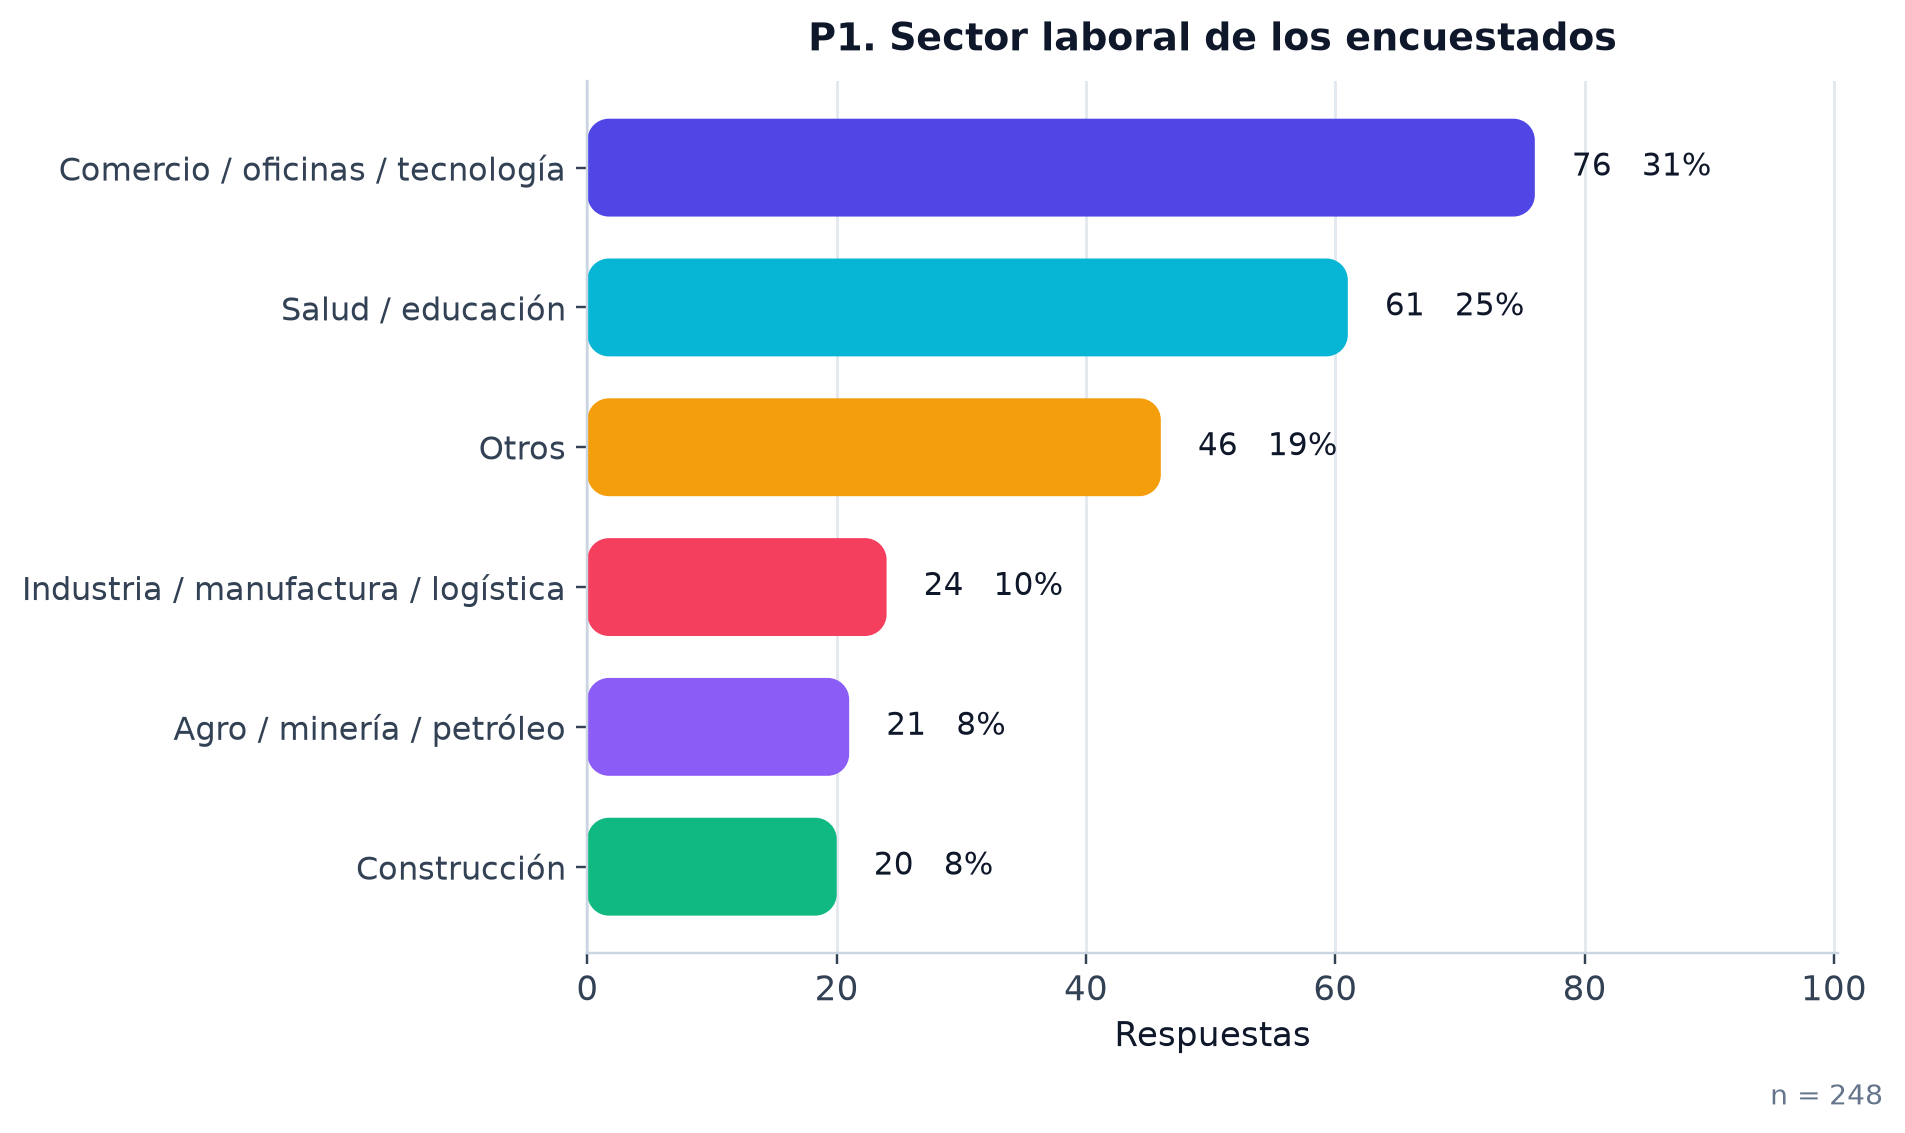
\includegraphics[width=0.92\textwidth]{figures/encuesta/p1_sector.png}
	\caption{\enc{Distribuci\'on por sector. Las categor\'{\i}as libres de baja frecuencia se agruparon en Otros. $n=248$.}}
	\label{fig:enc-p1}
\end{figure}

\enc{Comercio, oficinas y tecnolog\'{\i}a, 31\,\%. Salud y educaci\'on, 25\,\%. Otros, 19\,\%. Industria y log\'{\i}stica, 10\,\%. Agro, miner\'{\i}a y petr\'oleo, 9\,\%. Construcci\'on, 8\,\%.}

\subsection*{P2: Tama\~no del establecimiento}

\begin{figure}[htbp]
	\centering
	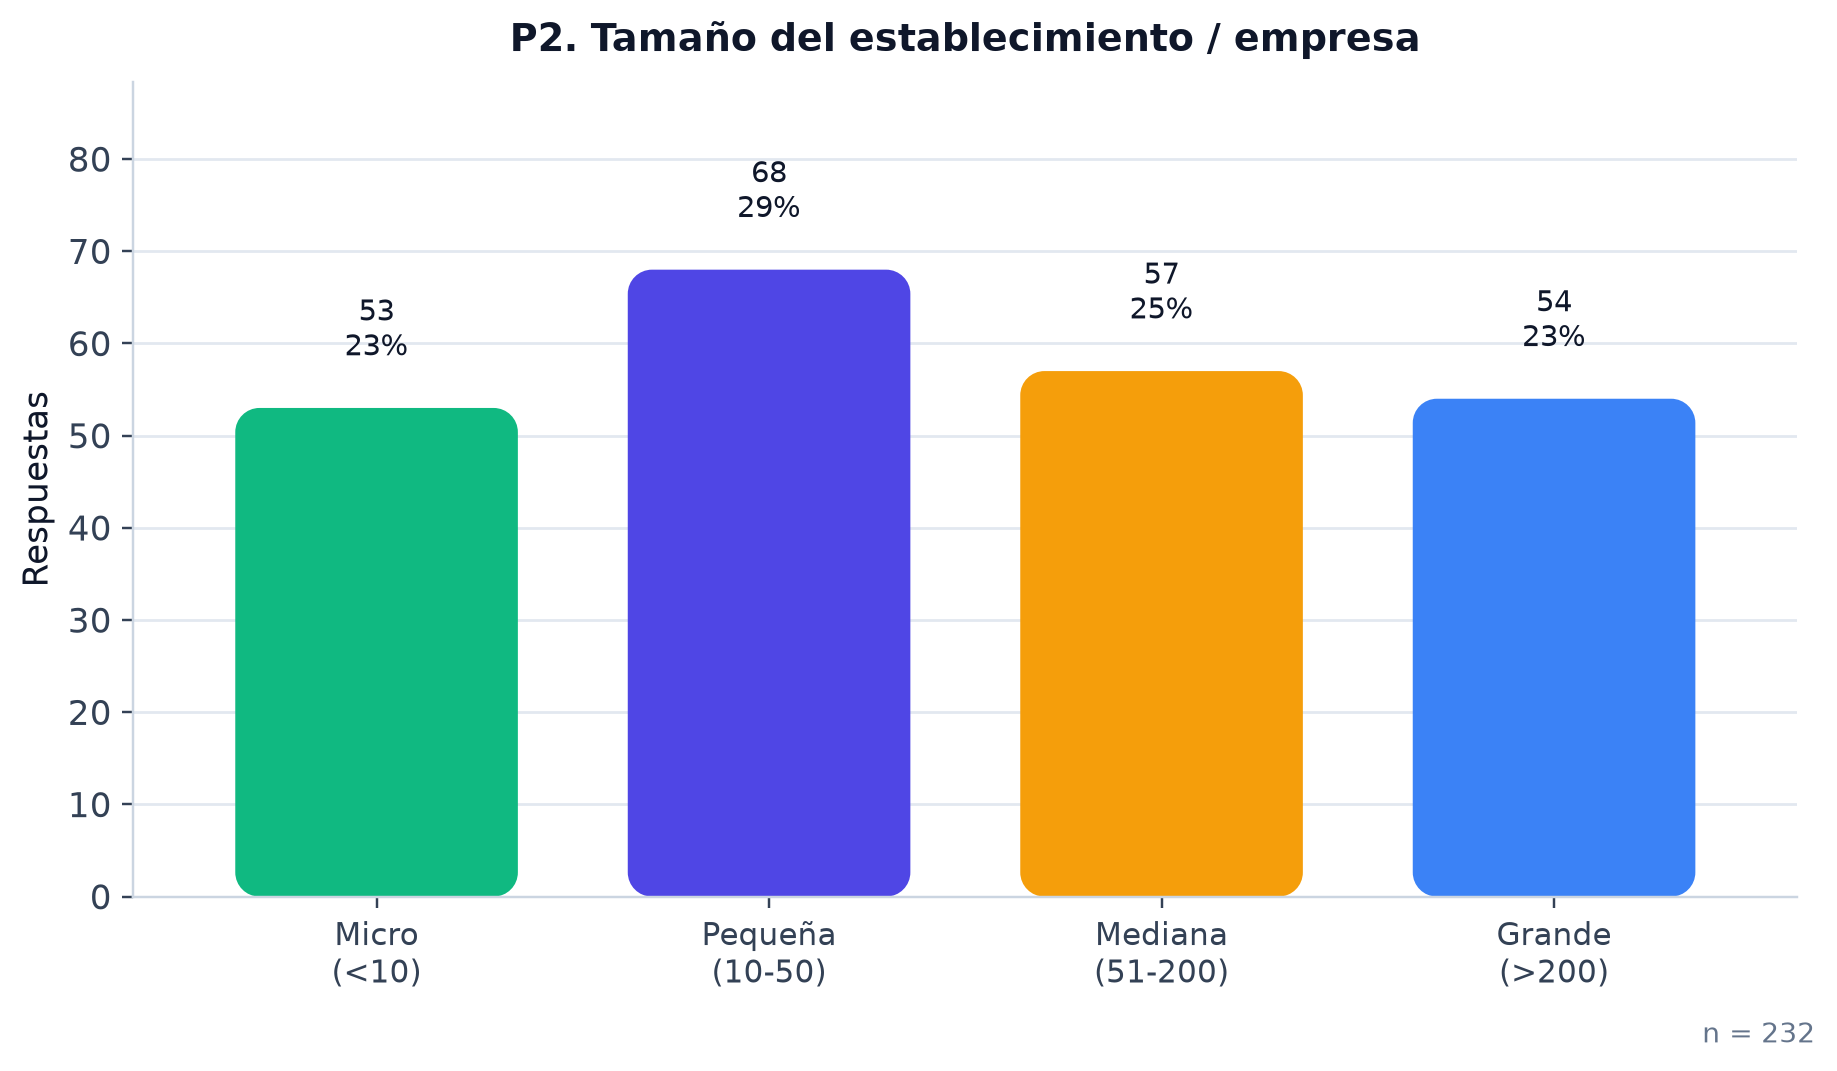
\includegraphics[width=0.92\textwidth]{figures/encuesta/p2_tamanio.png}
	\caption{\enc{Tama\~no aproximado de la empresa o establecimiento. $n=232$.}}
	\label{fig:enc-p2}
\end{figure}

\enc{Micro, 23\,\%. Peque\~na, 29\,\%. Mediana, 25\,\%. Gran empresa, 23\,\%.
Diecis\'eis respuestas de P1 no informaron tama\~no.}

\subsection*{P3: Conocimiento de la ART y auditor\'{\i}as}

\begin{figure}[htbp]
	\centering
	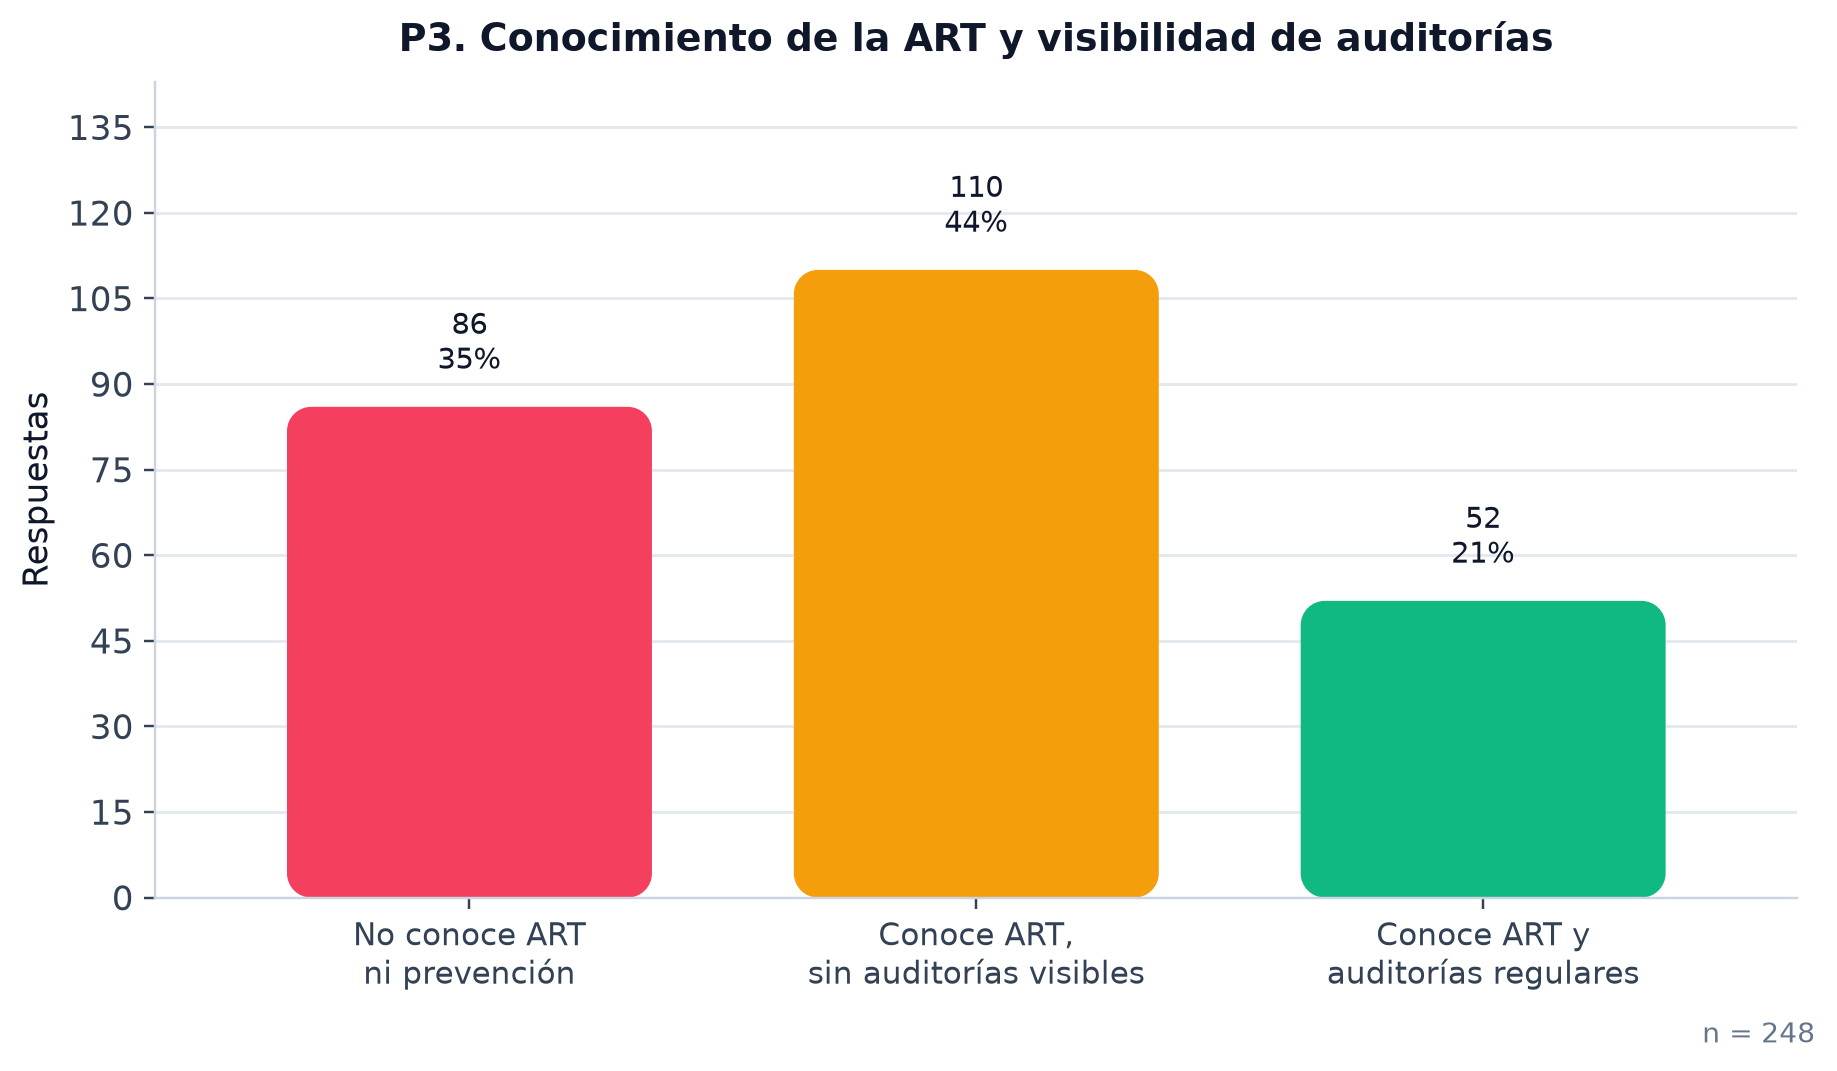
\includegraphics[width=0.92\textwidth]{figures/encuesta/p3_art.png}
	\caption{\enc{Conocimiento de la ART y visibilidad de auditor\'{\i}as preventivas. $n=248$.}}
	\label{fig:enc-p3}
\end{figure}

\enc{El 35\,\% no tiene idea de qu\'e ART lo cubre ni si hay prevenci\'on.
El 44\,\% conoce la ART pero nunca vio auditor\'{\i}as o inspecciones.
El 21\,\% conoce la ART y reporta auditor\'{\i}as regulares.}

\subsection*{P4: Capacitaciones y medidas de seguridad}

\begin{figure}[htbp]
	\centering
	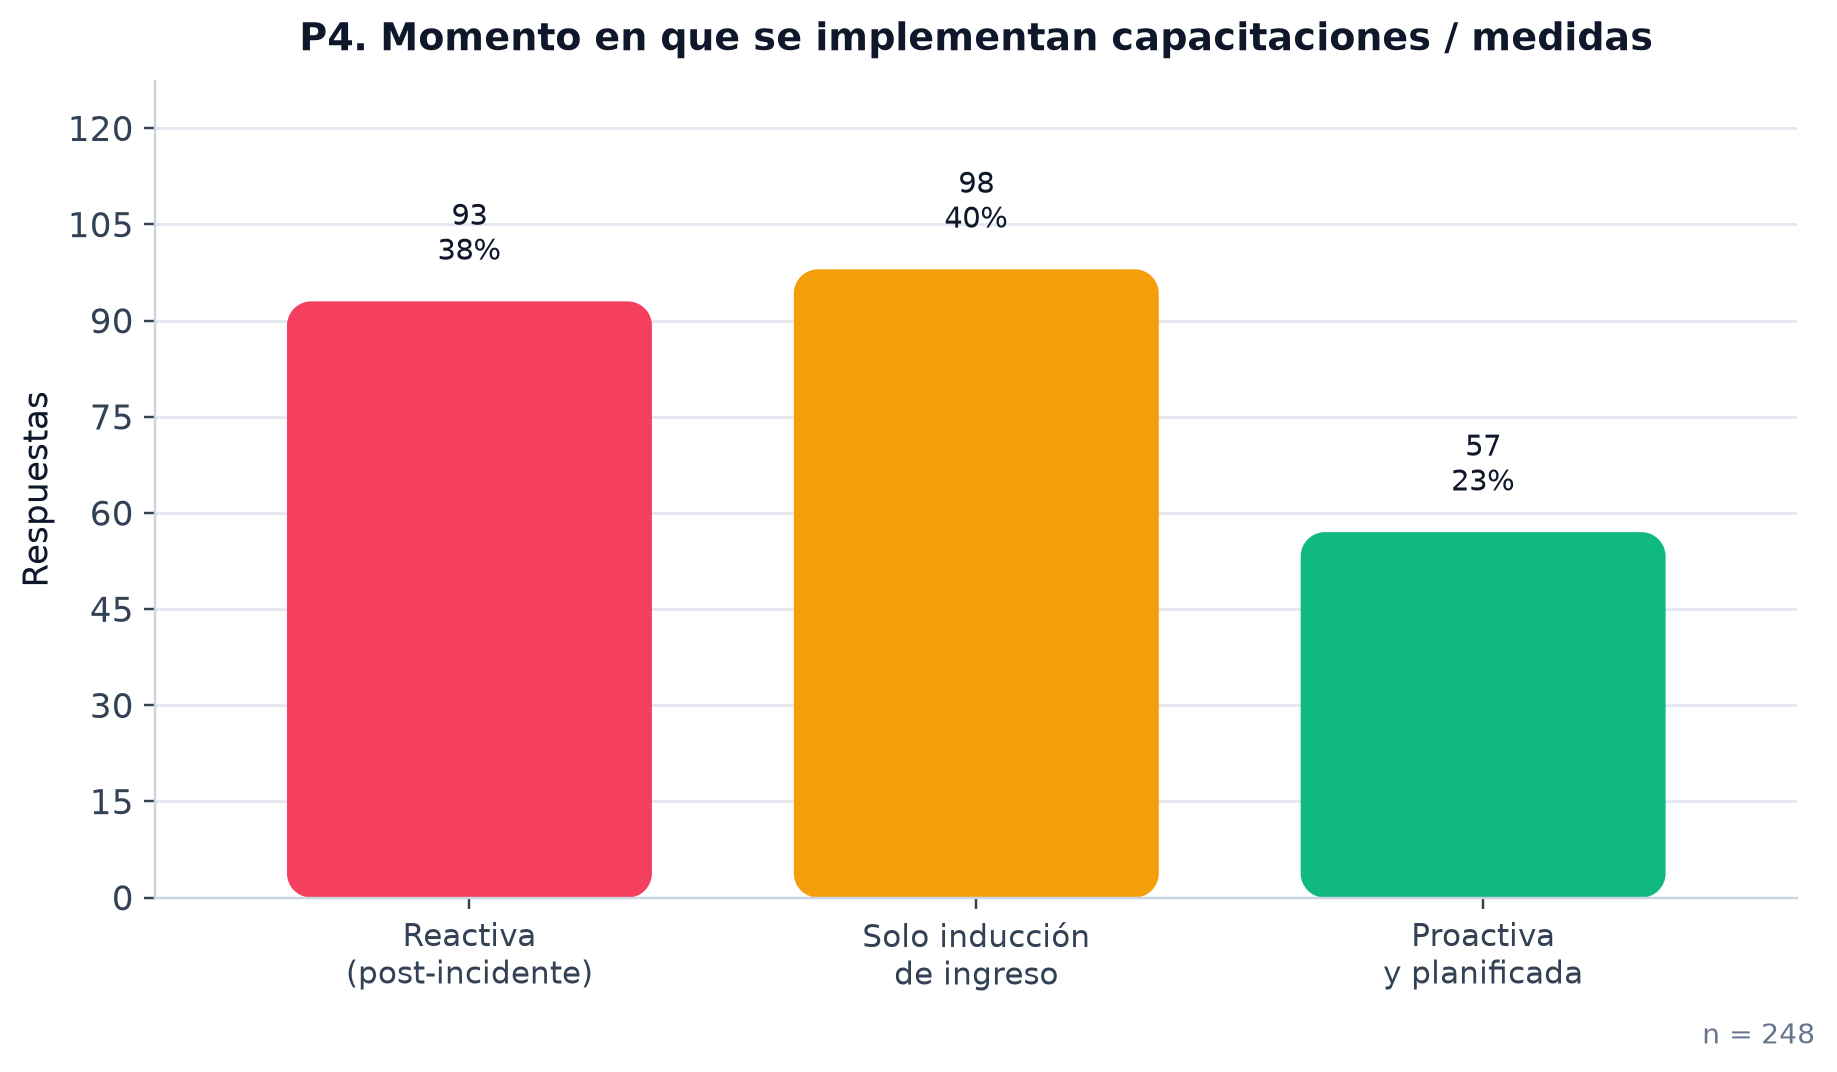
\includegraphics[width=0.92\textwidth]{figures/encuesta/p4_capacitaciones.png}
	\caption{\enc{Momento predominante de implementaci\'on de capacitaciones o medidas. $n=248$.}}
	\label{fig:enc-p4}
\end{figure}

\enc{El 38\,\% las sit\'ua despu\'es de un incidente.
El 40\,\% las limita a la inducci\'on de ingreso.
El 23\,\% describe un enfoque proactivo y planificado a lo largo del a\~no.}

\subsection*{P5: Preparaci\'on percibida, escala 1 a 5}

\begin{figure}[htbp]
	\centering
	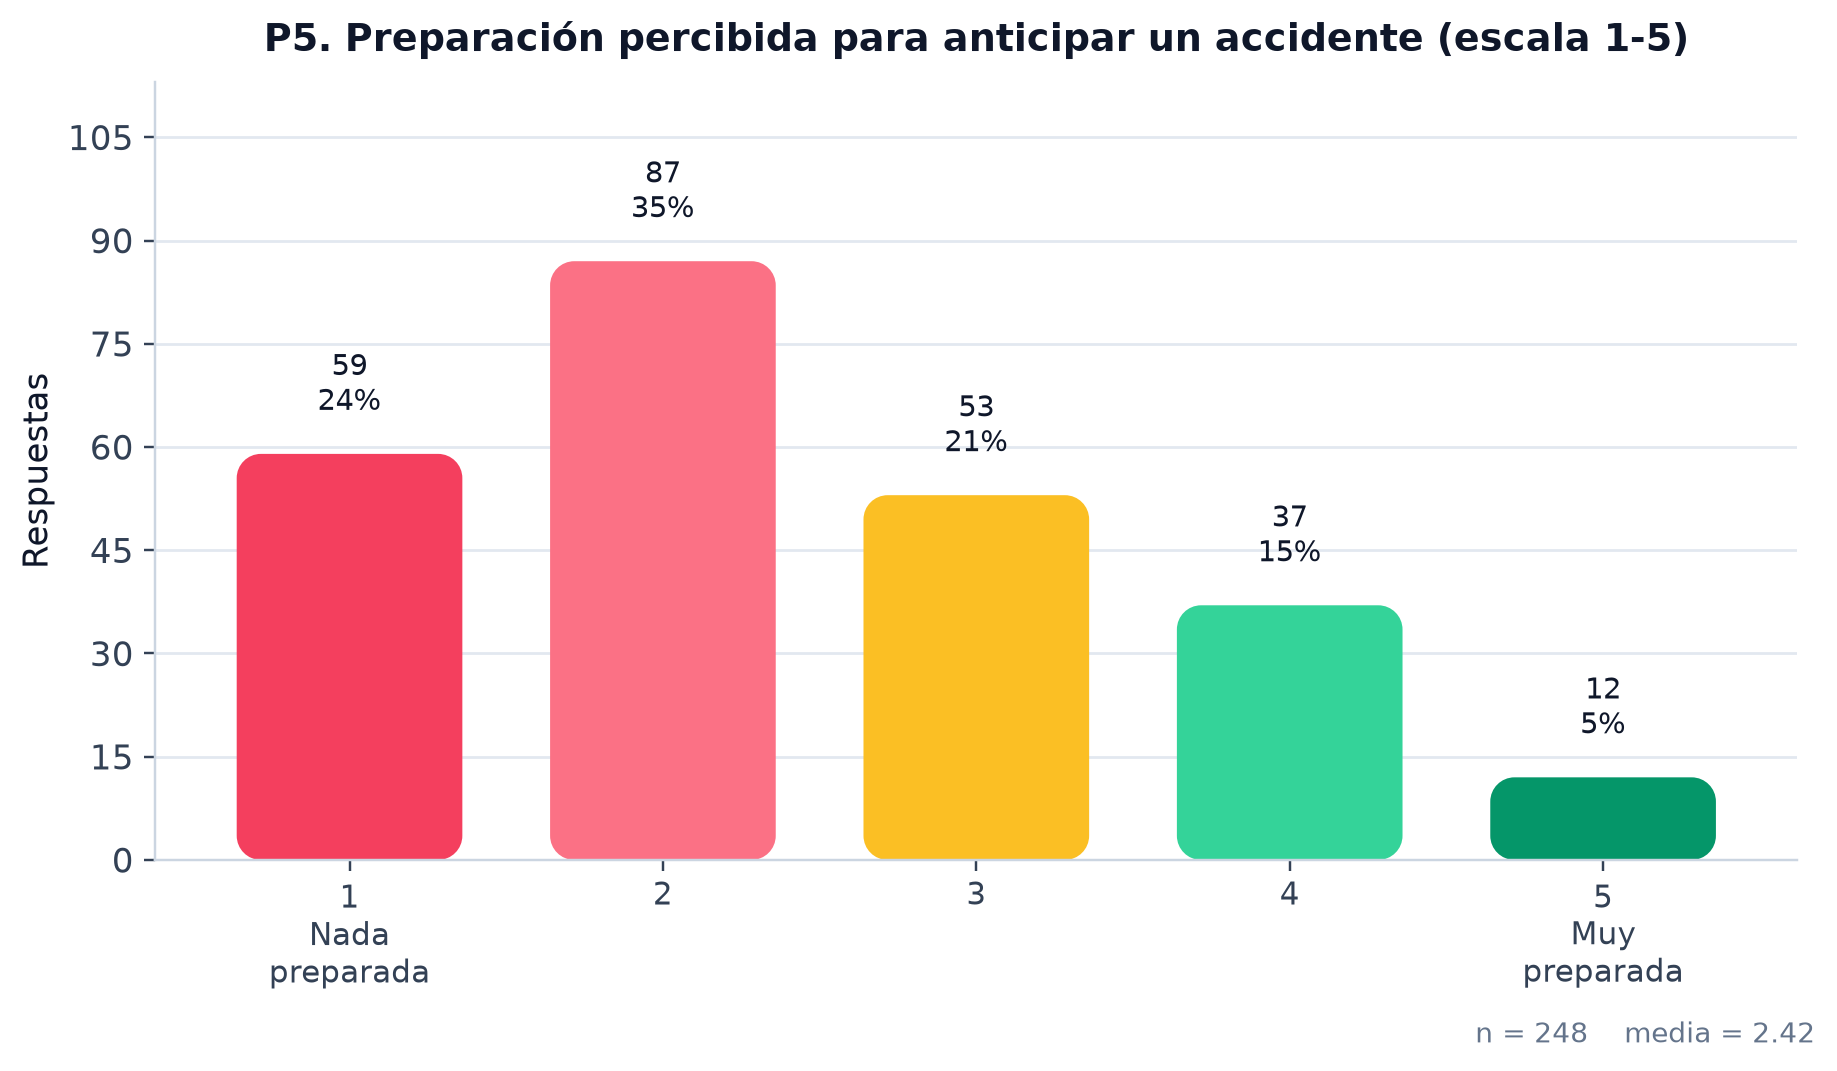
\includegraphics[width=0.92\textwidth]{figures/encuesta/p5_preparacion.png}
	\caption{\enc{Autoevaluaci\'on de preparaci\'on de la empresa para anticipar un accidente. $n=248$; media 2,42.}}
	\label{fig:enc-p5}
\end{figure}

\enc{Media 2,42. Mediana 2.
El 59\,\% elige 1 o 2.
El 5\,\% elige el m\'aximo, 5.}

\subsection*{P6: Experiencia de accidente o enfermedad profesional}

\begin{figure}[htbp]
	\centering
	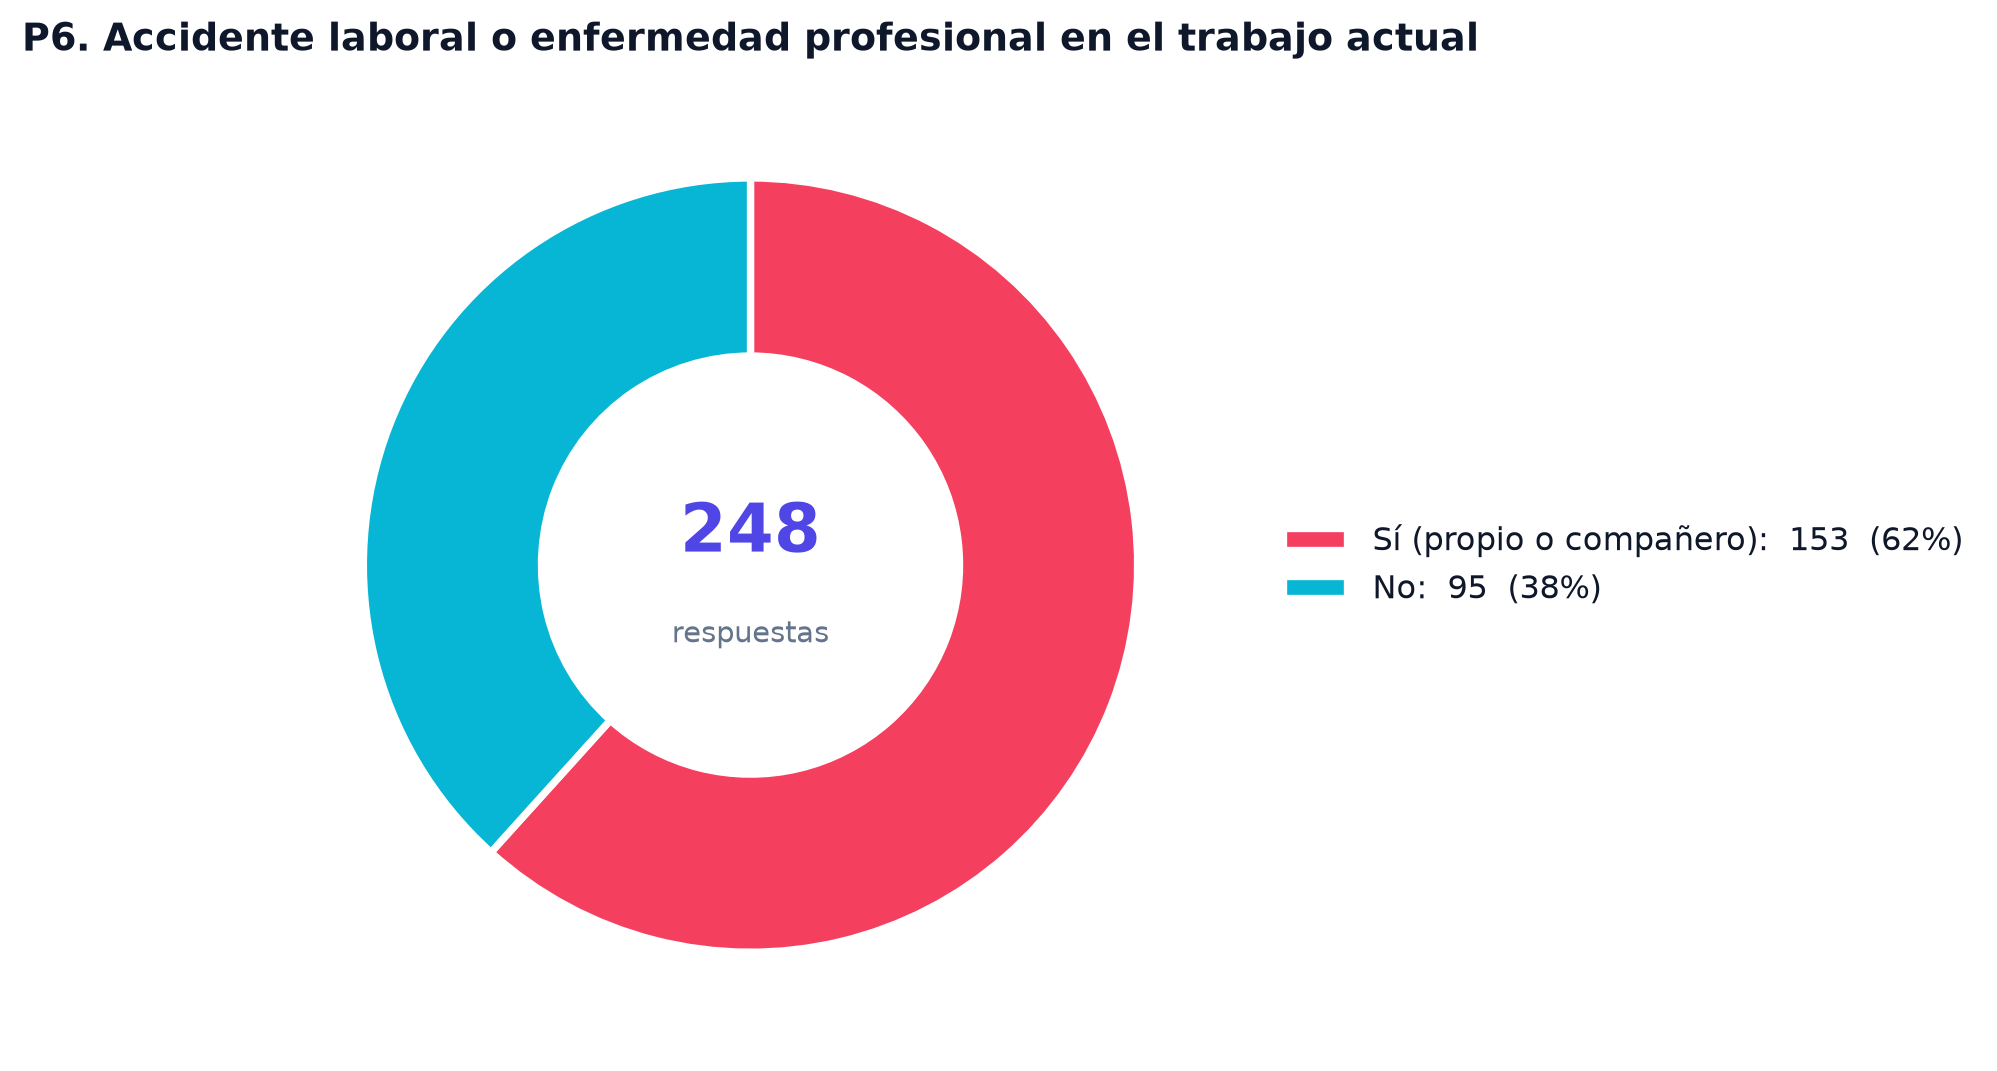
\includegraphics[width=0.88\textwidth]{figures/encuesta/p6_accidente.png}
	\caption{\enc{Experiencia de accidente laboral o enfermedad profesional, propio o de un compa\~nero. $n=248$.}}
	\label{fig:enc-p6}
\end{figure}

\enc{El 62\,\% reporta al menos un episodio en el trabajo actual.}

\subsection*{P7: Cambios operativos tras el accidente}

\begin{figure}[htbp]
	\centering
	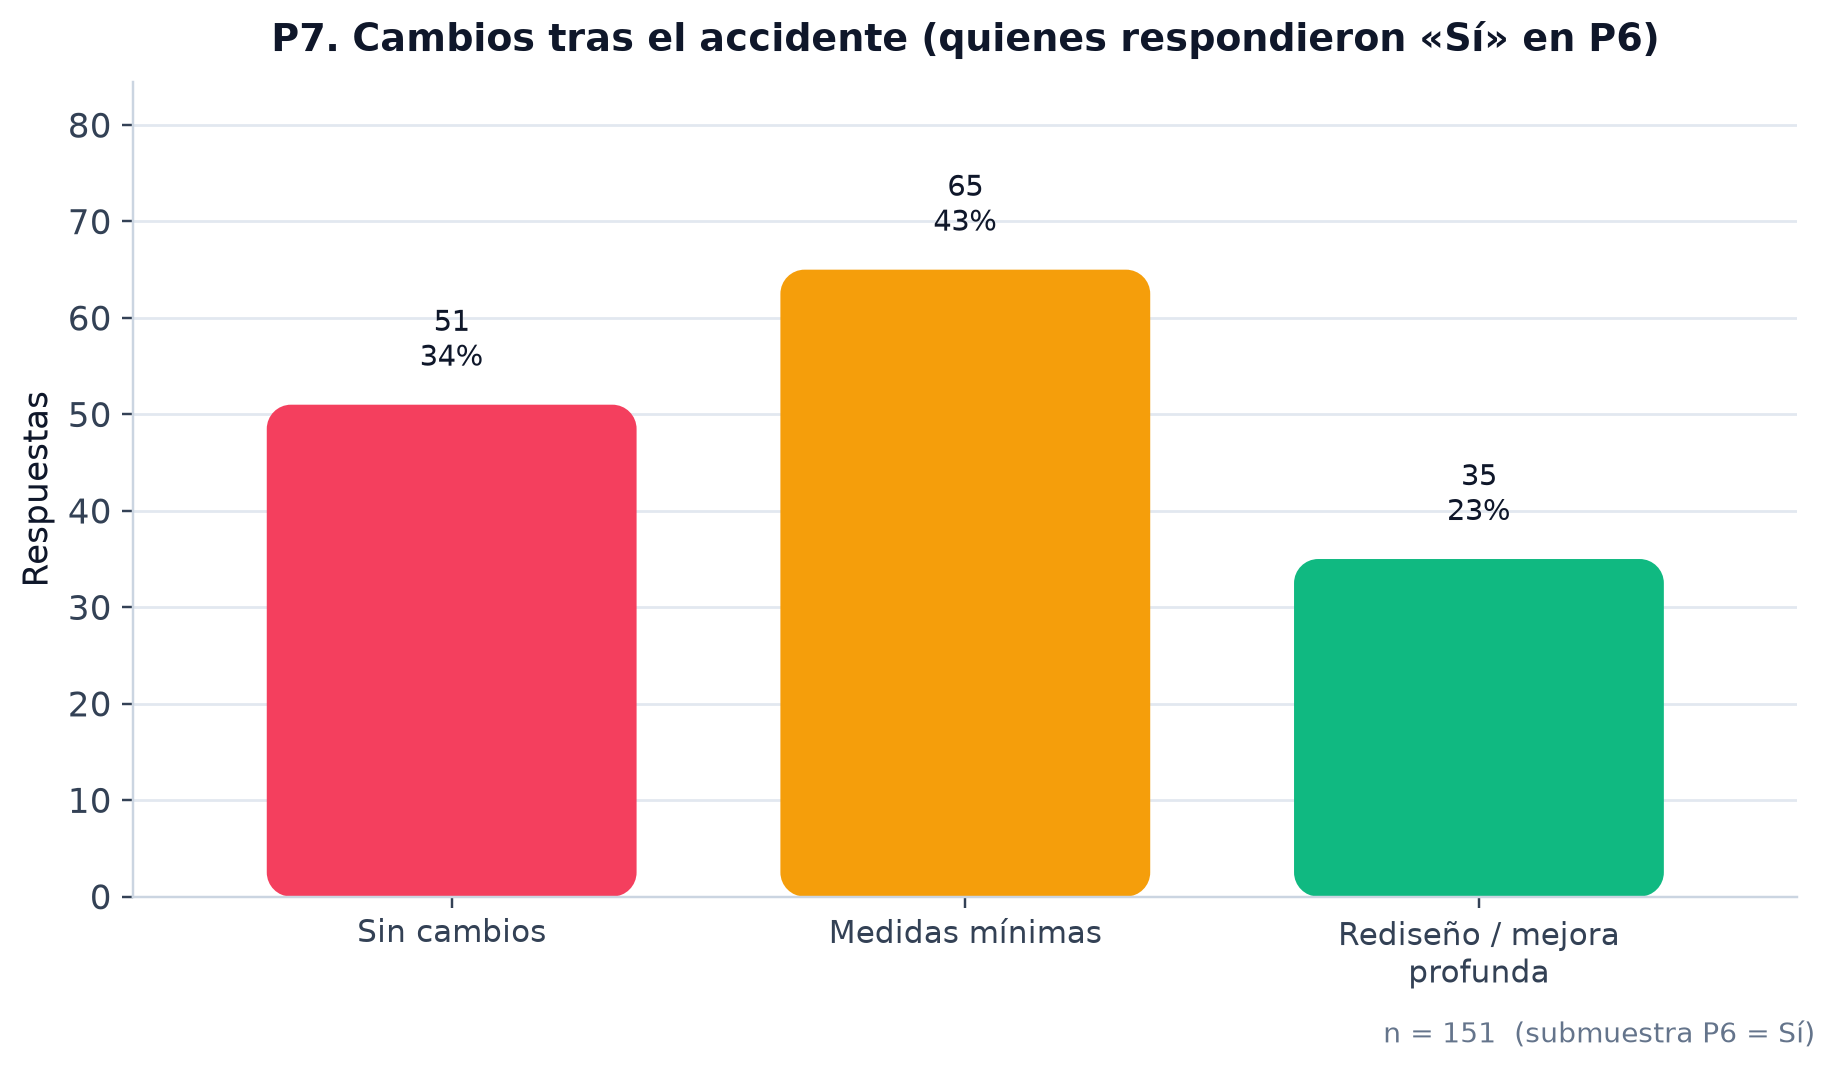
\includegraphics[width=0.92\textwidth]{figures/encuesta/p7_cambios.png}
	\caption{\enc{Cambios percibidos tras el accidente, solo quienes respondieron S\'{\i} en P6. $n=151$ v\'alidas, tras excluir No aplica residuales.}}
	\label{fig:enc-p7}
\end{figure}

\enc{El 23\,\% percibi\'o redise\~no de procesos y mejora de seguridad.
El 34\,\% indica que todo sigui\'o igual.
El 43\,\% solo medidas m\'{\i}nimas, charla o cartel.}

\subsection*{Limitaciones}

Muestra de conveniencia, sin marco muestral ART o SRT.
Autoreporte perceptivo, no auditor\'{\i}a objetiva de visitas.
Posible sesgo por las redes de difusi\'on del formulario.
